\documentclass[12pt,a4paper,portrait]{article}

\usepackage[portuguese]{babel} 	% hifenização
\usepackage[utf8]{inputenc} 	% acentos e cedilhas
\usepackage[T1]{fontenc} 		% evitar problemas com fonts
\usepackage{graphicx}
\usepackage{graphicx,wrapfig}
\usepackage{fancyhdr}
\usepackage{lastpage}
\usepackage[dvipsnames]{xcolor}
\usepackage{colortbl}
\usepackage{enumerate}			% Include the enumerate-package
\usepackage{listings}           % Include the listings-package
\usepackage{color}				% Include the color-package
\usepackage{askmaps}
\usepackage{booktabs}
\usepackage{xcolor}

\usepackage{babel}
\usepackage[font=small,labelfont=bf]{caption}

\pagestyle{fancy}
\fancyhf{}
\rhead{Engenharia Informática 2º Ano}
\lhead{ISMAT}
\rfoot{Página \thepage \hspace{1pt} de \pageref{LastPage}}

\setcounter{secnumdepth}{5}	% actualiza o contador máximo de níveis para subsections
\setcounter{tocdepth}{5}	% actualiza o contador máximo de níveis na Tabela de Conteudo

\begin{document}
	\begin{titlepage}
	\begin{center}
	
		% Upper part of the page. The '~' is needed because \\
		% only works if a paragraph has started.
		%
\includegraphics[width=0.95\textwidth]{./logo}~\\[1,5cm]
		
\includegraphics{./logo}
		% \includegraphics{logo_ismat}
		
		
		%\textsc{\LARGE Instituto Superior Manuel Teixeira Gomes }\\[1.5cm]
		
		\textsc{\Large Algoritmia e Estrutura de Dados}\\[1.5cm]
		
		% Title
		\newcommand{\HRule}{\rule{\linewidth}{0.5mm}}
		\HRule \\[0.4cm]
		{ \huge \bfseries Travel Salesman Problem \\[0.4cm] }
		
		\HRule \\[1.5cm]
		
		% discente e docente
		\noindent
		
		\begin{minipage}[t]{0.4\textwidth}
			\begin{flushleft} \large
				\emph{Discente(s):}\\
				Pedro \textsc{Roldan}\\
				Leandro \textsc{Moreira}\\
			\end{flushleft}
		\end{minipage}%
		\begin{minipage}[t]{0.4\textwidth}
			\begin{flushright} \large
				\emph{Docente:} \\
				Doutor Faroq \textsc{AlTam}
			\end{flushright}
		\end{minipage}
		
		\vfill
		
		% Bottom of the page
		{\large \today}
	
	\end{center}
\end{titlepage}
	\tableofcontents
	
	\lstdefinestyle{customc}{
	  belowcaptionskip=1\baselineskip,
	  breaklines=true,
	  frame=L,
	  xleftmargin=\parindent,
	  language=C,
	  showstringspaces=false,
	  basicstyle=\footnotesize\ttfamily,
	  keywordstyle=\bfseries\color{green!40!black},
	  commentstyle=\itshape\color{purple!40!black},
	  identifierstyle=\color{blue},
	  stringstyle=\color{orange},
      tabsize=1,
	}
	
	\newpage
	\section{Introdução}
		O travel salesman problem (TSP) é um problema bastante comum largamente encontrado em diversas aplicações tais como: empresas de transporte (e.g. UPS), escalas de tripulação de companhias aéreas, etc.\\
		Em principio, um vendedor necessita de efetuar uma viagem por diversas cidades, onde inicia a viagem numa determinada cidade (Casa), visita todas as cidades para vender os seus produtos, e retorna a casa.\\
		\subsection{Requisitos Minimos}	
			O TSP pode ser representado por uma lista de nós, sendo o objetivo descobrir uma serie de caminhos (Edges) entre cada um dos nós.\\\\
			Sendo que:\\
			\begin{itemize}
				\item Cada nó (Cidade) pode ser visitado apenas 1 vez.
				\item Os caminhos formam uma Tour.
				\item O custo da Tour deve ser o mínimo possível.
			\end{itemize}
			A tour TSP é um gráfico direcionado, onde cada nó representa uma cidade, e cada edge representa um caminho entre 2 cidades.\\
			Cada edge têm um peso, que é no seu caso mais simples a distancia euclidiana entre os seus nós.\\
			Este peso pode ser composto por diversos fatores, no entanto neste projeto apenas se considera a distancia entre nós.\\ 			
			\newpage
	\section{2-Opt} \label{ssec:num1}
			O algoritmo 2-Opt foi proposto por Croes em 1958, embora o movimento básico tenha sido sugerido por Flood em 1956.\\ 
			O algoritmo 2-Opt basicamente remove 2 nós (Edges) da tour, e conecta os dois caminhos criados. Isto é normalmente referido como um movimento 2-Opt.\\
			\subsection{Técnica 2-Opt}	
			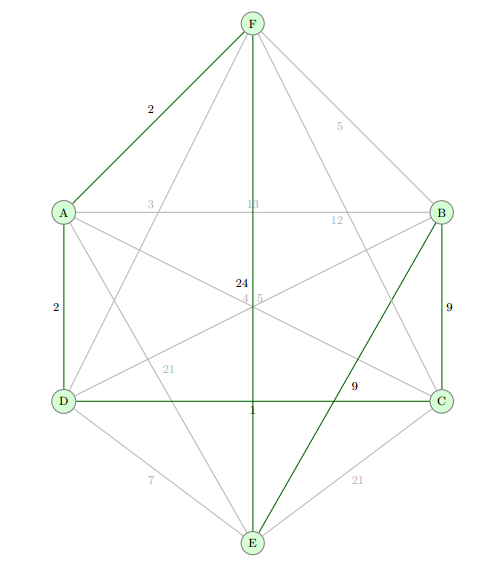
\includegraphics[width=1.0\textwidth]{imagens/1}
			Aqui vamos utilizar uma lista de 6 nós, em que a distancia total da tour é de 47.\\
			\newpage
			Em primeiro lugar selecionamos um edge, neste caso \textbf{AD}, vamos de seguida selecionar outro edge que não seja adjacente ao egde em uso,\textbf{AD}.\\
			Neste exemplo apenas dispomos de um edge possível \textbf{BE}.\\
			Podemos assim trocar \textbf{AD} e \textbf{BE} por \textbf{AB} e \textbf{BE}.\\
			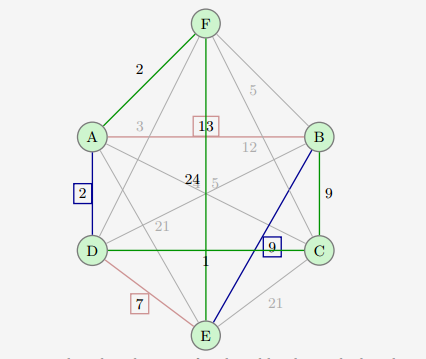
\includegraphics[width=1.0\textwidth]{imagens/2}
			No entanto, a soma das distancias dos edges possíveis de trocar é \textbf{maior} que a soma das distancias dos edges originais. Assim sendo não trocamos os edges.\\
			\newpage
			Considerando o próximo edge \textbf{DC}, apenas dispõe de 1 edge não-adjacente,
			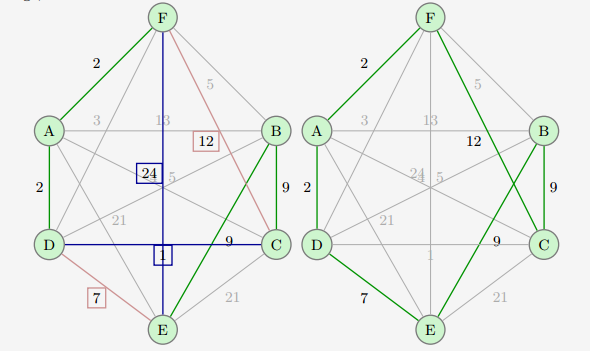
\includegraphics[width=1.0\textwidth]{imagens/3}
			Aqui, como a soma das distancias dos edges originais é \textbf{maior} que a soma das distancias dos edges possíveis de trocar, efetuamos a troca de edges.\\\\
			\newpage
			Considerando o edge \textbf{DE}, este edge dispõe do edge não-adjacente \textbf{CF}.\\
			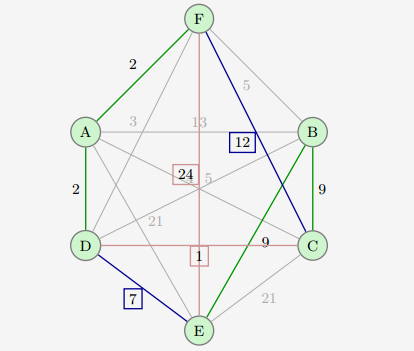
\includegraphics[width=1.0\textwidth]{imagens/4}
			Como a soma das distancias dos edges possíveis de trocar são maiores que a soma das distancias dos edges originais, não se efetua trocas.\\\\
			\newpage
			No proximo passo o edge selecionado é \textbf{EB}.O edge não-adjacente a este edge é \textbf{FA}.\\
			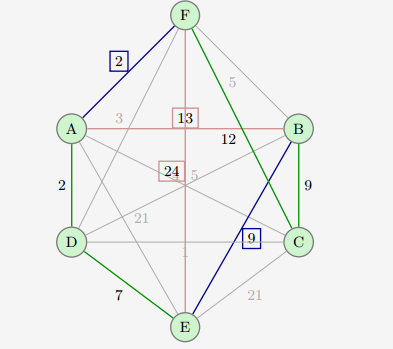
\includegraphics[width=1.0\textwidth]{imagens/5}
			Não é necessário efetuar trocas de edges.\\\\
			\newpage
			Vamos selecionar o próximo edge, \textbf{BC}.O edge não-adjacente a este é \textbf{AD}.
			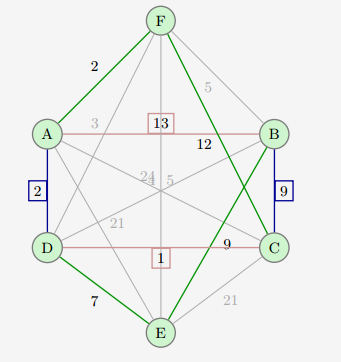
\includegraphics[width=1.0\textwidth]{imagens/6}
			Este cenário não garante alterações ao caminho.\\\\
			\newpage
			Agora vamos considerar o edge \textbf{CF}.O edge não-adjacente a este é \textbf{DE}\\
			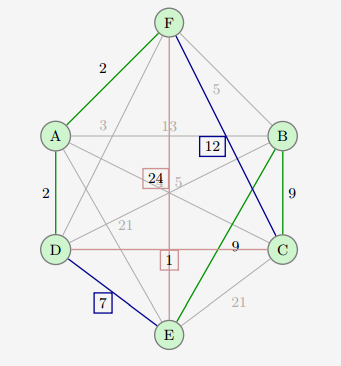
\includegraphics[width=1.0\textwidth]{imagens/7}
			Aqui, não é necessário efetuar alterações ao caminho visto que a soma da distancia dos edges possíveis de trocar é inferior quando comparado com os edges existentes.\\\\
			\newpage
			O proximo edge a ser considerado é  \textbf{FA}. O edge não adjacente é \textbf{EB}.\\
			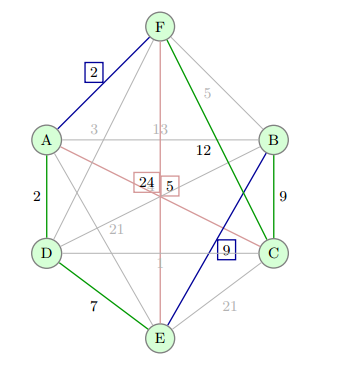
\includegraphics[width=1.0\textwidth]{imagens/8}
			Este também é um caso em que não existe necessidade de se efetuar trocas de edges.\\\\
			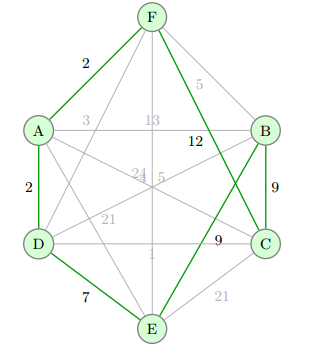
\includegraphics[width=1.0\textwidth]{imagens/9}
			Finalmente chegamos a uma solução optimizada. A solução apresenta um custo de 41, efetivamente inferior ao custo da solução inicial.\\\\
			\newpage
	\section{Enquadramento}
	O trabalho descrito neste relatório foi realizado recorrendo à linguagem de programação ANSI C, assim como os recursos disponibilizados na unidade curricular.\\
		\subsection{Motivação}
			A principal motivação para a realização deste trabalho, resulta da importância em implementar o algoritmo 2-Opt ao problema Travel Salesman, assim como demonstrar os conhecimentos alcançados na disciplina de Algoritmia e Estrutura de Dados.\\
		\subsection{Objectivos}
			Pretende-se através deste trabalho, atingir uma solução válida para o Travel Salesman Problem, implementando o algoritmo 2-Opt.\\
	\section{Conclusões}
		A implementação do algoritmo 2-Opt ao TSP desenvolvida, para além de permitir os requisitos pedidos no enunciado do trabalho prático, permite também a possível implementação de outros algoritmos,pois sendo modular torna-se mais escalável, entre outras funcionalidades.\\
		De frisar que devido à liberdade proporcionada, quer na sua forma de desenvolvimento quer na implementação permitiu desta forma aguçar a curiosidade para o uso de diversos algoritmos para a solução do Travel Salesman Problem.\\
		Foi sem duvida um desafio interessante, mas que por limitação de tempo, deixa ainda uma larga margem para melhoramentos.\\
	\newpage
	\section{Bibliografia}
	\bibliographystyle{plain}
	\bibliography{./bibliotecas}

	\newpage
	\section{Anexos}
		Ficheiro "relatorio.pdf" e "eps.c, eps.h, tsp.c, tsp.h, file.c, file.h, main.c", assim como as pastas "tspdata, results", compactado num ficheiro "trabalho.zip".\\\\
		Não existem quaisquer códigos ou listagens adicionais.\\					
\end{document}          
